\documentclass[10pt, handout]{beamer}

\usepackage[english]{babel}
\usepackage{times}
\usepackage{rotating}
\usepackage{graphicx}
\usepackage{amssymb,amsmath,mathtools,multirow}
\usepackage[ansinew]{inputenc}
\usepackage[tikz]{bclogo}


%\usepackage[utf8]{inputenc}
\usepackage[cyr]{aeguill}
%\usepackage[T1]{fontenc}
\usetheme{Antibes}
%\useoutertheme{infolines}

\title{The (In)stability of Reg-Arima Estimations } 
\author{
D. Ladiray, A. Quartier-la-Tente
\thanks{Contact email: dominique.ladiray@insee.fr}
}
\date{SACE 04-10-2018, Riga}

\setbeamertemplate{navigation symbols}{}
\addtobeamertemplate{navigation symbols}{}{%
    \usebeamerfont{footline}%
    \usebeamercolor[fg]{footline}%
    \hspace{1em}%
    \insertframenumber/\inserttotalframenumber
}
\begin{document}
 \addtobeamertemplate{title page}{\includegraphics[height=1cm, width=10.8cm]{img/SACELogo.png}}{}

\begin{frame}
\titlepage
\end{frame}
\begin{frame}{Outline}
  \tableofcontents
\end{frame}

\section{Introduction}

\begin{frame}{Never, never forget\ldots{}}
\begin{center}
\huge
``All models are false, but some are useful'' 
\end{center}
\normalsize
\vskip \baselineskip
George E. P. Box 
\vskip \baselineskip 
\vskip \baselineskip 

\footnotesize
Box, G.E.P. (1979), ``Robustness in the Strategy of Scientific Model Building'', in R.L. Launer and G.N. Wilkinson (eds.), Robustness in Statistics: Proceedings of a Workshop, Academic Press.
\normalsize
\end{frame}


\begin{frame}{The 2-Step Seasonal Adjustment Procedure}
 \centering
 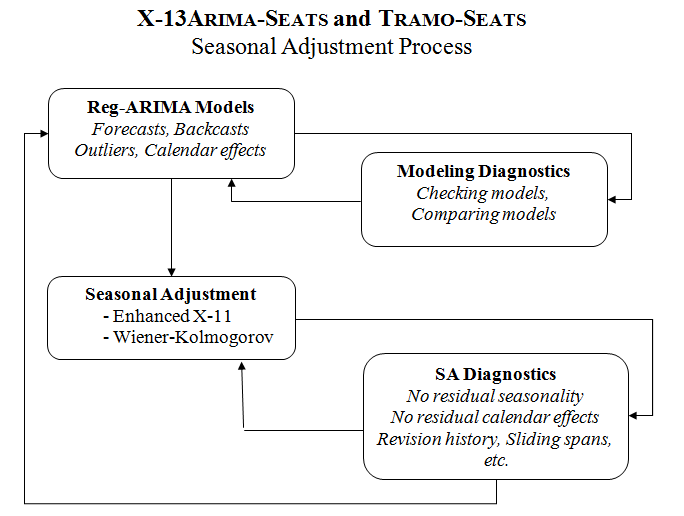
\includegraphics[height = 0.8\textheight]{img/X13-TSmethods.png}
\end{frame}

\begin{frame}{Reg-ARIMA modelling}

The Reg-ARIMA Model commonly used in SA can be written:

\[
 \begin{drcases}
\text{Additive: }& Y_t \\
\text{Multiplicative: }& \log(Y_t) 
\end{drcases} 
= \underbrace{\beta_0 LY_t + \beta_1 WD_t}_{\text{WD regressors}} + 
\underbrace{\sum_{i}\gamma_iO_{i,t}}_{\mathclap{\text{outliers}}} + \underbrace{\varepsilon_t}_{\sim ARIMA}
\]
\vskip \baselineskip
\pause
The main objective of the presentation is to illustrate potential instability problems in the estimations. We focus on 3 examples: 
\begin{itemize}
 \item Leap Year effect
 \item Outliers estimates
 \item Identification of the ARIMA model
\end{itemize}
\end{frame}

\section{Estimation of the Leap-Year Effect}
\begin{frame}{Outline}
\tableofcontents[currentsection, hideothersubsections]
\end{frame}

\subsection{How and when carry out the leap year
adjustment?}

\begin{frame}{The Leap-Year Effect}
 \begin{itemize}
  \item The Gregorian calendar is a solar calendar where the length of the year is supposed to represent the time the Earth takes to make a complete revolution around the Sun. 
	\item To achieve this equality on the long run, a day is added to February if the year is divisible by 4 but not by 100, unless the year is also divisible by 400.
  \item The Leap-Year effect is therefore a calendar effect which estimates the impact of this extra day.
	\item[]
	\item<2-> According to the ``ESS Guidelines on SA'':
    \begin{itemize}
	     \item<2-> CA should be done for those time series for which there is an economic rationale for the existence of calendar effects and statistical evidence. 
	     \item<2-> Moreover, CA should not result in frequent large revisions when additional data become available, if it does, it is an indication that the method's estimates are not reliable.
    \end{itemize}
 \end{itemize}
\end{frame}

\begin{frame}{Estimation of the Leap-Year Effect}
Two main methods:
\begin{enumerate}
\item<1-> Using the Reg-ARIMA model with a specific regressor:
\[
LY_t = \begin{cases}
0.75 & \text{for leap year Februaries} \\
-0.25  & \text{for non leap year Februaries} \\
0 & \text{Otherwise}
\end{cases}
\]
\item<2-> Pre-adjustment of February values (X12-ARIMA, see Bell[1992]): 
\[\begin{cases}
\frac{28.25}{29} \simeq 0.974 & \text{for leap year Februaries} \\
\frac{28.25}{28} \simeq 1.009 & \text{for non leap year Februaries} \\
1 & \text{Otherwise}
\end{cases}
\]
\end{enumerate}
\end{frame}

\subsection{Methodology of the study}
\begin{frame}{Methodology (1/2)}
To assess the quality of the Leap Year estimate using Reg-Arima model, we use the following methodology:
\begin{itemize}
	\item We use the European monthly industrial production indexes and turnover indexes (NACE rev. 2 at 2, 3 and 4 digits).
		\begin{itemize}
		  \item These series are likely to present a leap year effect. We focus on the 2 198 series longer than 12 years only.
	  \end{itemize}
	\item Step 1: For each series the decomposition model, the ARIMA model, outliers and trading-day effects are identified and estimated on the complete span.
	\item<2-> Step 2: Then, the reg-ARIMA model is re-estimated on the 48 first observations.
	\item<2-> Step 3: The process is repeated adding each time a new observation. Thus, for a 13-year series, we will obtain $12 \times 13 - 48 = 108$ estimations of the LY coefficient.
\end{itemize}
\end{frame}

\begin{frame}{Methodology (2/2)}
\begin{itemize}
	\item These simulations allows studying the convergence of the LY coefficient.
	\item We assume that the convergence is reached when: (1) the LY coefficient remains positive (2) significant and (3) when the last estimations are not statistically different.
	\item Other specifications have been tested (changing the first estimation period, ARIMA model not fixed etc.) with similar results.
	\item We present here the results for the 410 IPI series which reached convergence.
\end{itemize}
\end{frame}

\subsection{Examples}
\begin{frame}{Examples (1/2)}
Series IPI FR-0610: extraction of crude petroleum.
\vskip \baselineskip
\centering
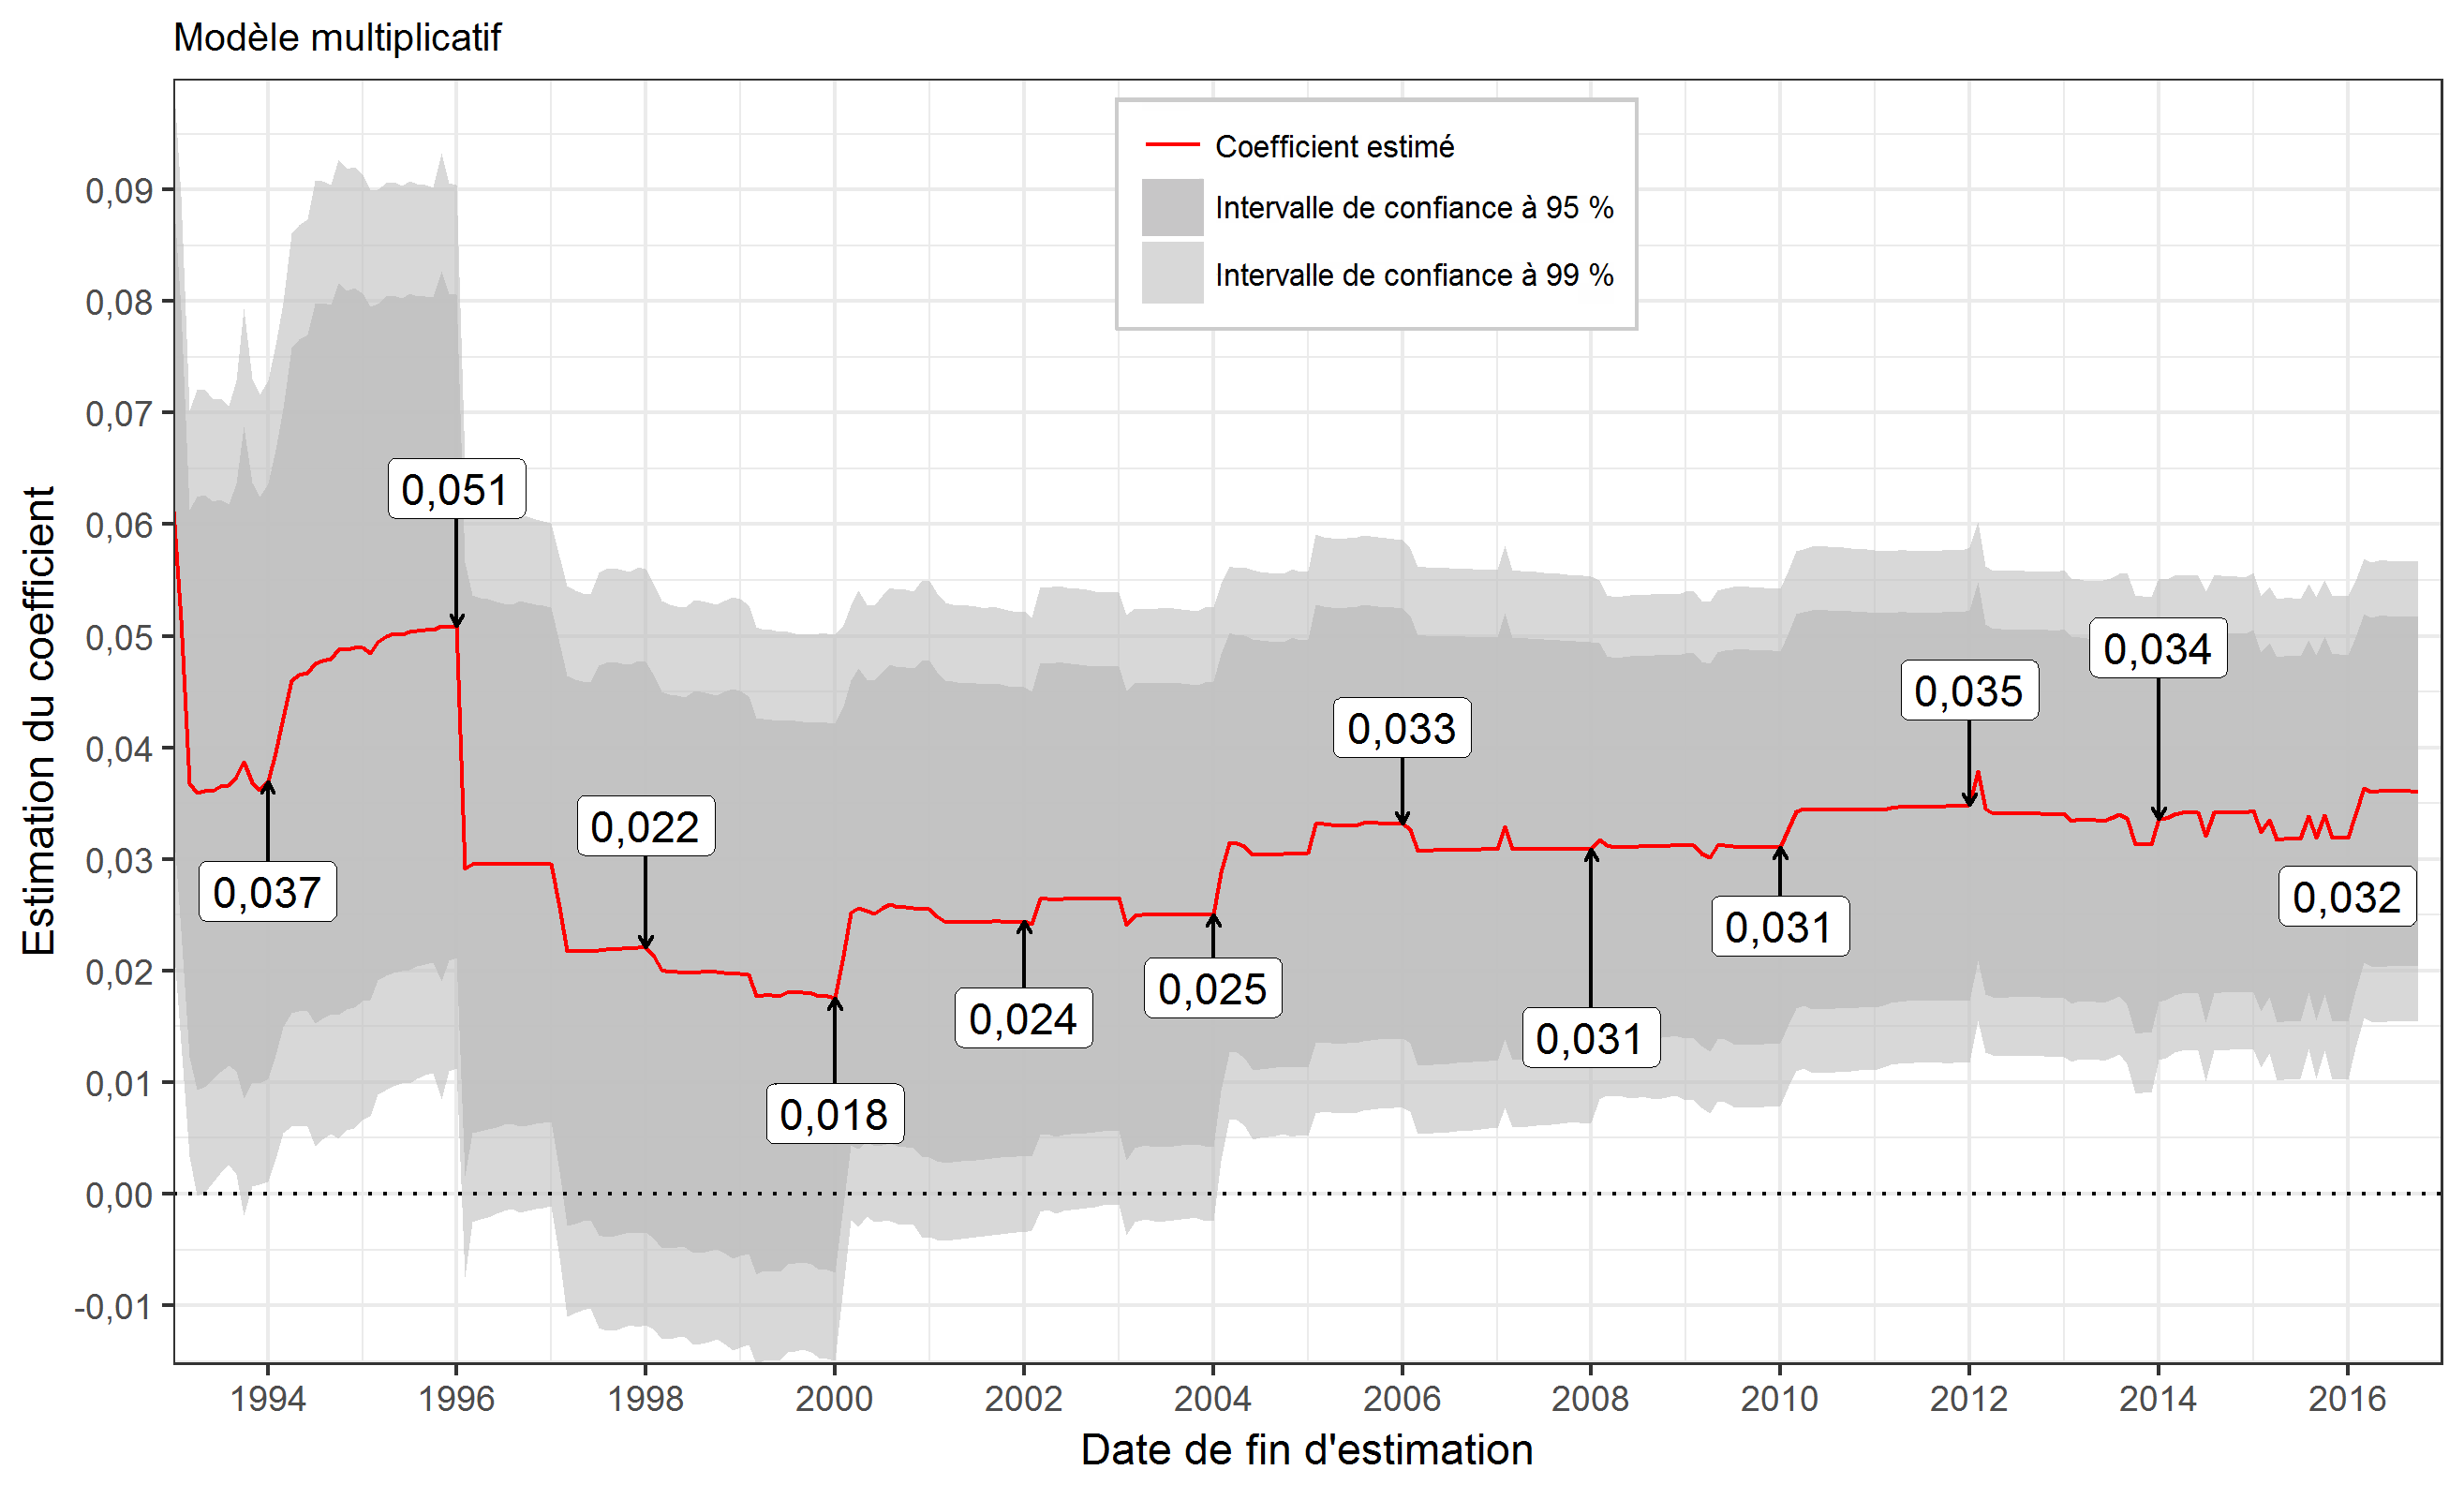
\includegraphics[width = 0.9\textwidth]{img/LYexemple1.png}
\end{frame}

\begin{frame}{Examples (2/2)}
Series IPI FR-1391: manufacture of knitted and crocheted fabrics.
\vskip \baselineskip
\centering
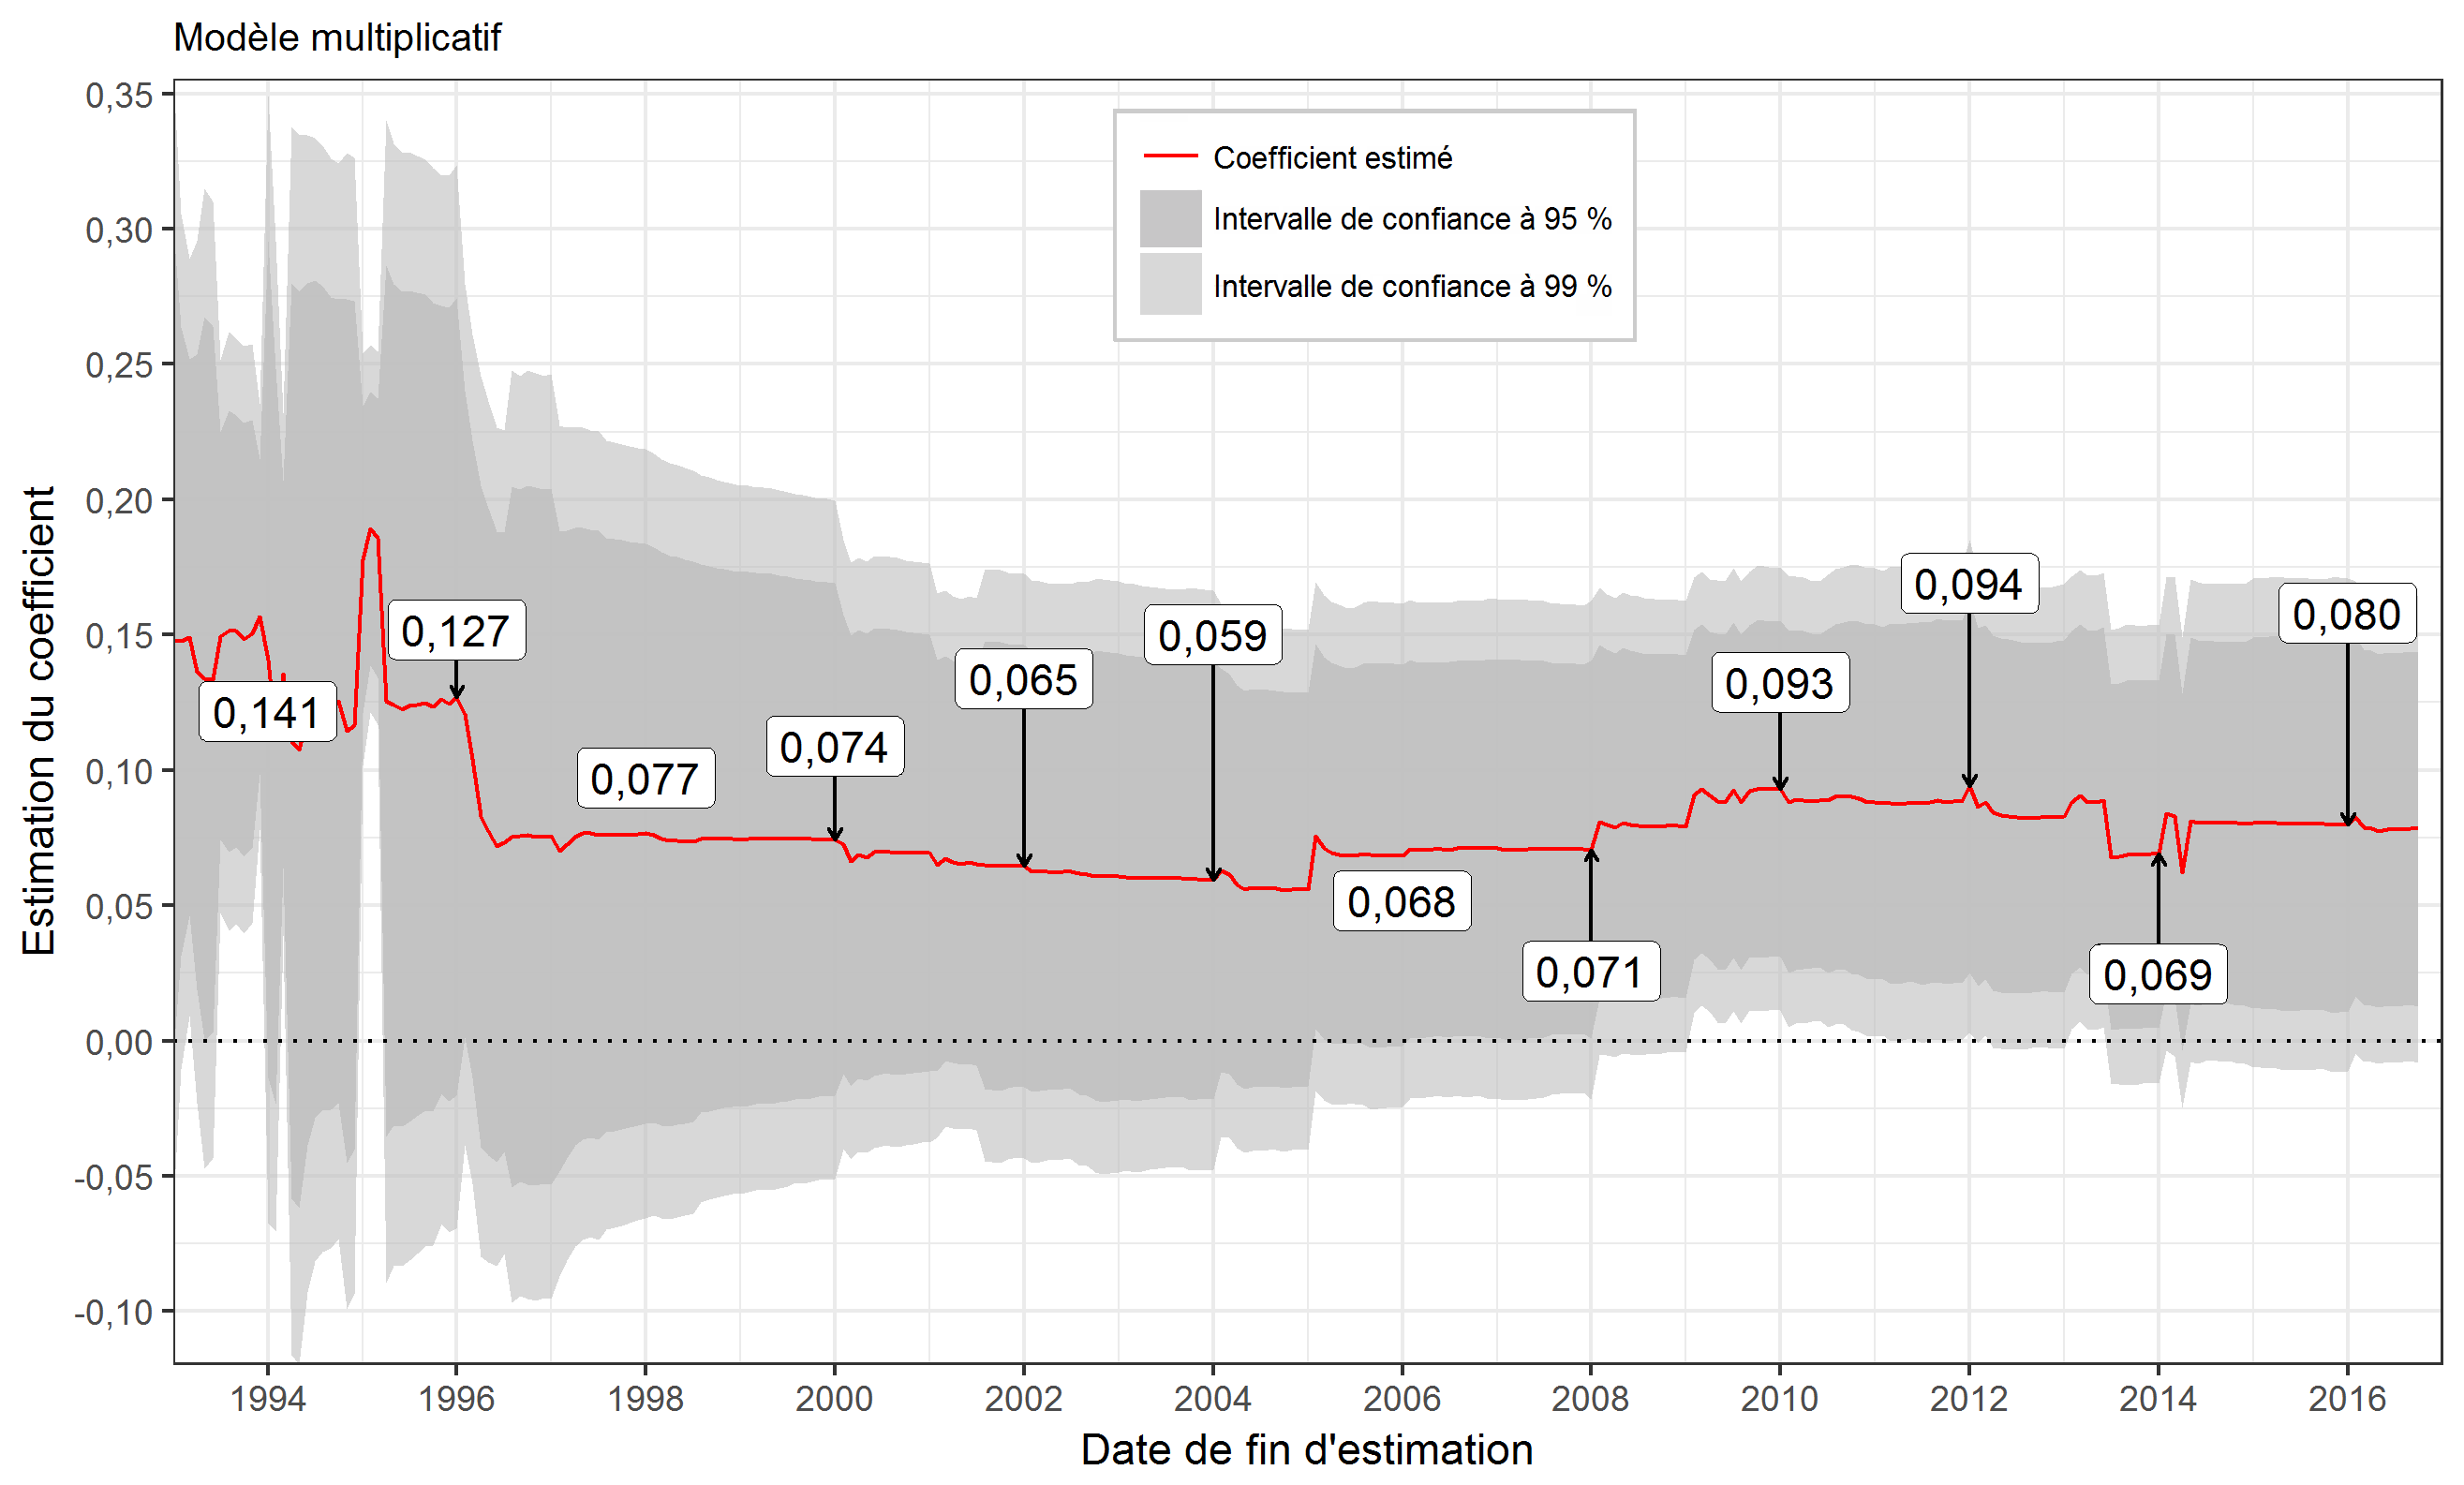
\includegraphics[width = 0.9\textwidth]{img/LYexemple2.png}
\end{frame}

\subsection{Results}
\begin{frame}{A pretty slow convergence\ldots{}}
\scriptsize
For 50\% of the series, more than 18 years of observations are required for the estimation to converge.
\vskip \baselineskip
\normalsize
 \centering
 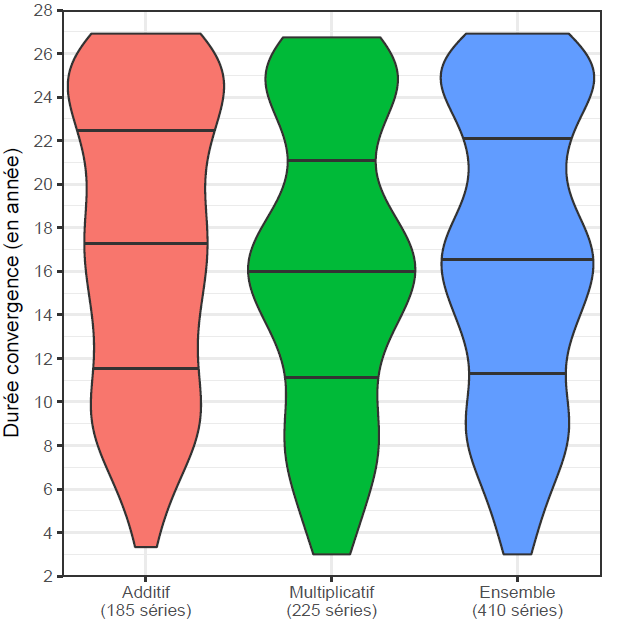
\includegraphics[height = 0.7\textheight]{img/LYconvergence.png}
\end{frame}

\begin{frame}{\ldots{} Towards a sometimes curious value}
\scriptsize
For at least 25\% of the series, the convergence value looks suspect.
\vskip \baselineskip
\normalsize
\centering
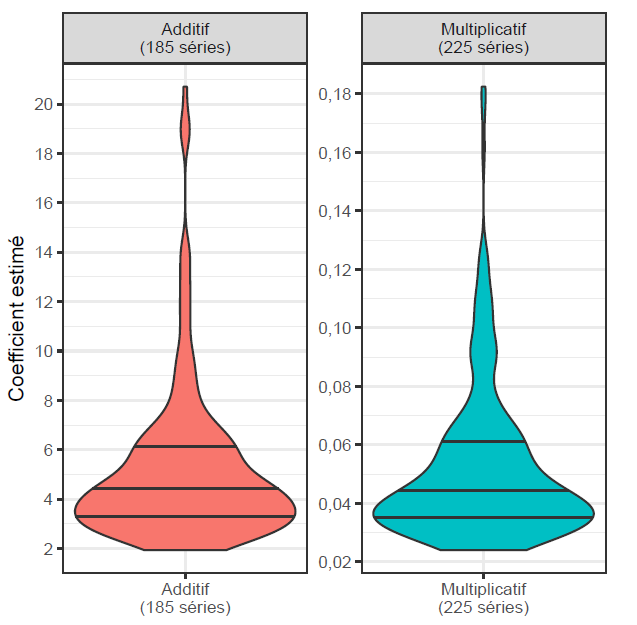
\includegraphics[height = 0.7\textheight]{img/LYvaleur.png}
\end{frame}

\begin{frame}{Comparison of the two correction methods}
\footnotesize
Percentage of series for which the AICC of the pre-adjustment method is lower than the AICC of the Reg-Arima method (on the 2 198 series).
\normalsize
\begin{figure}
\centering
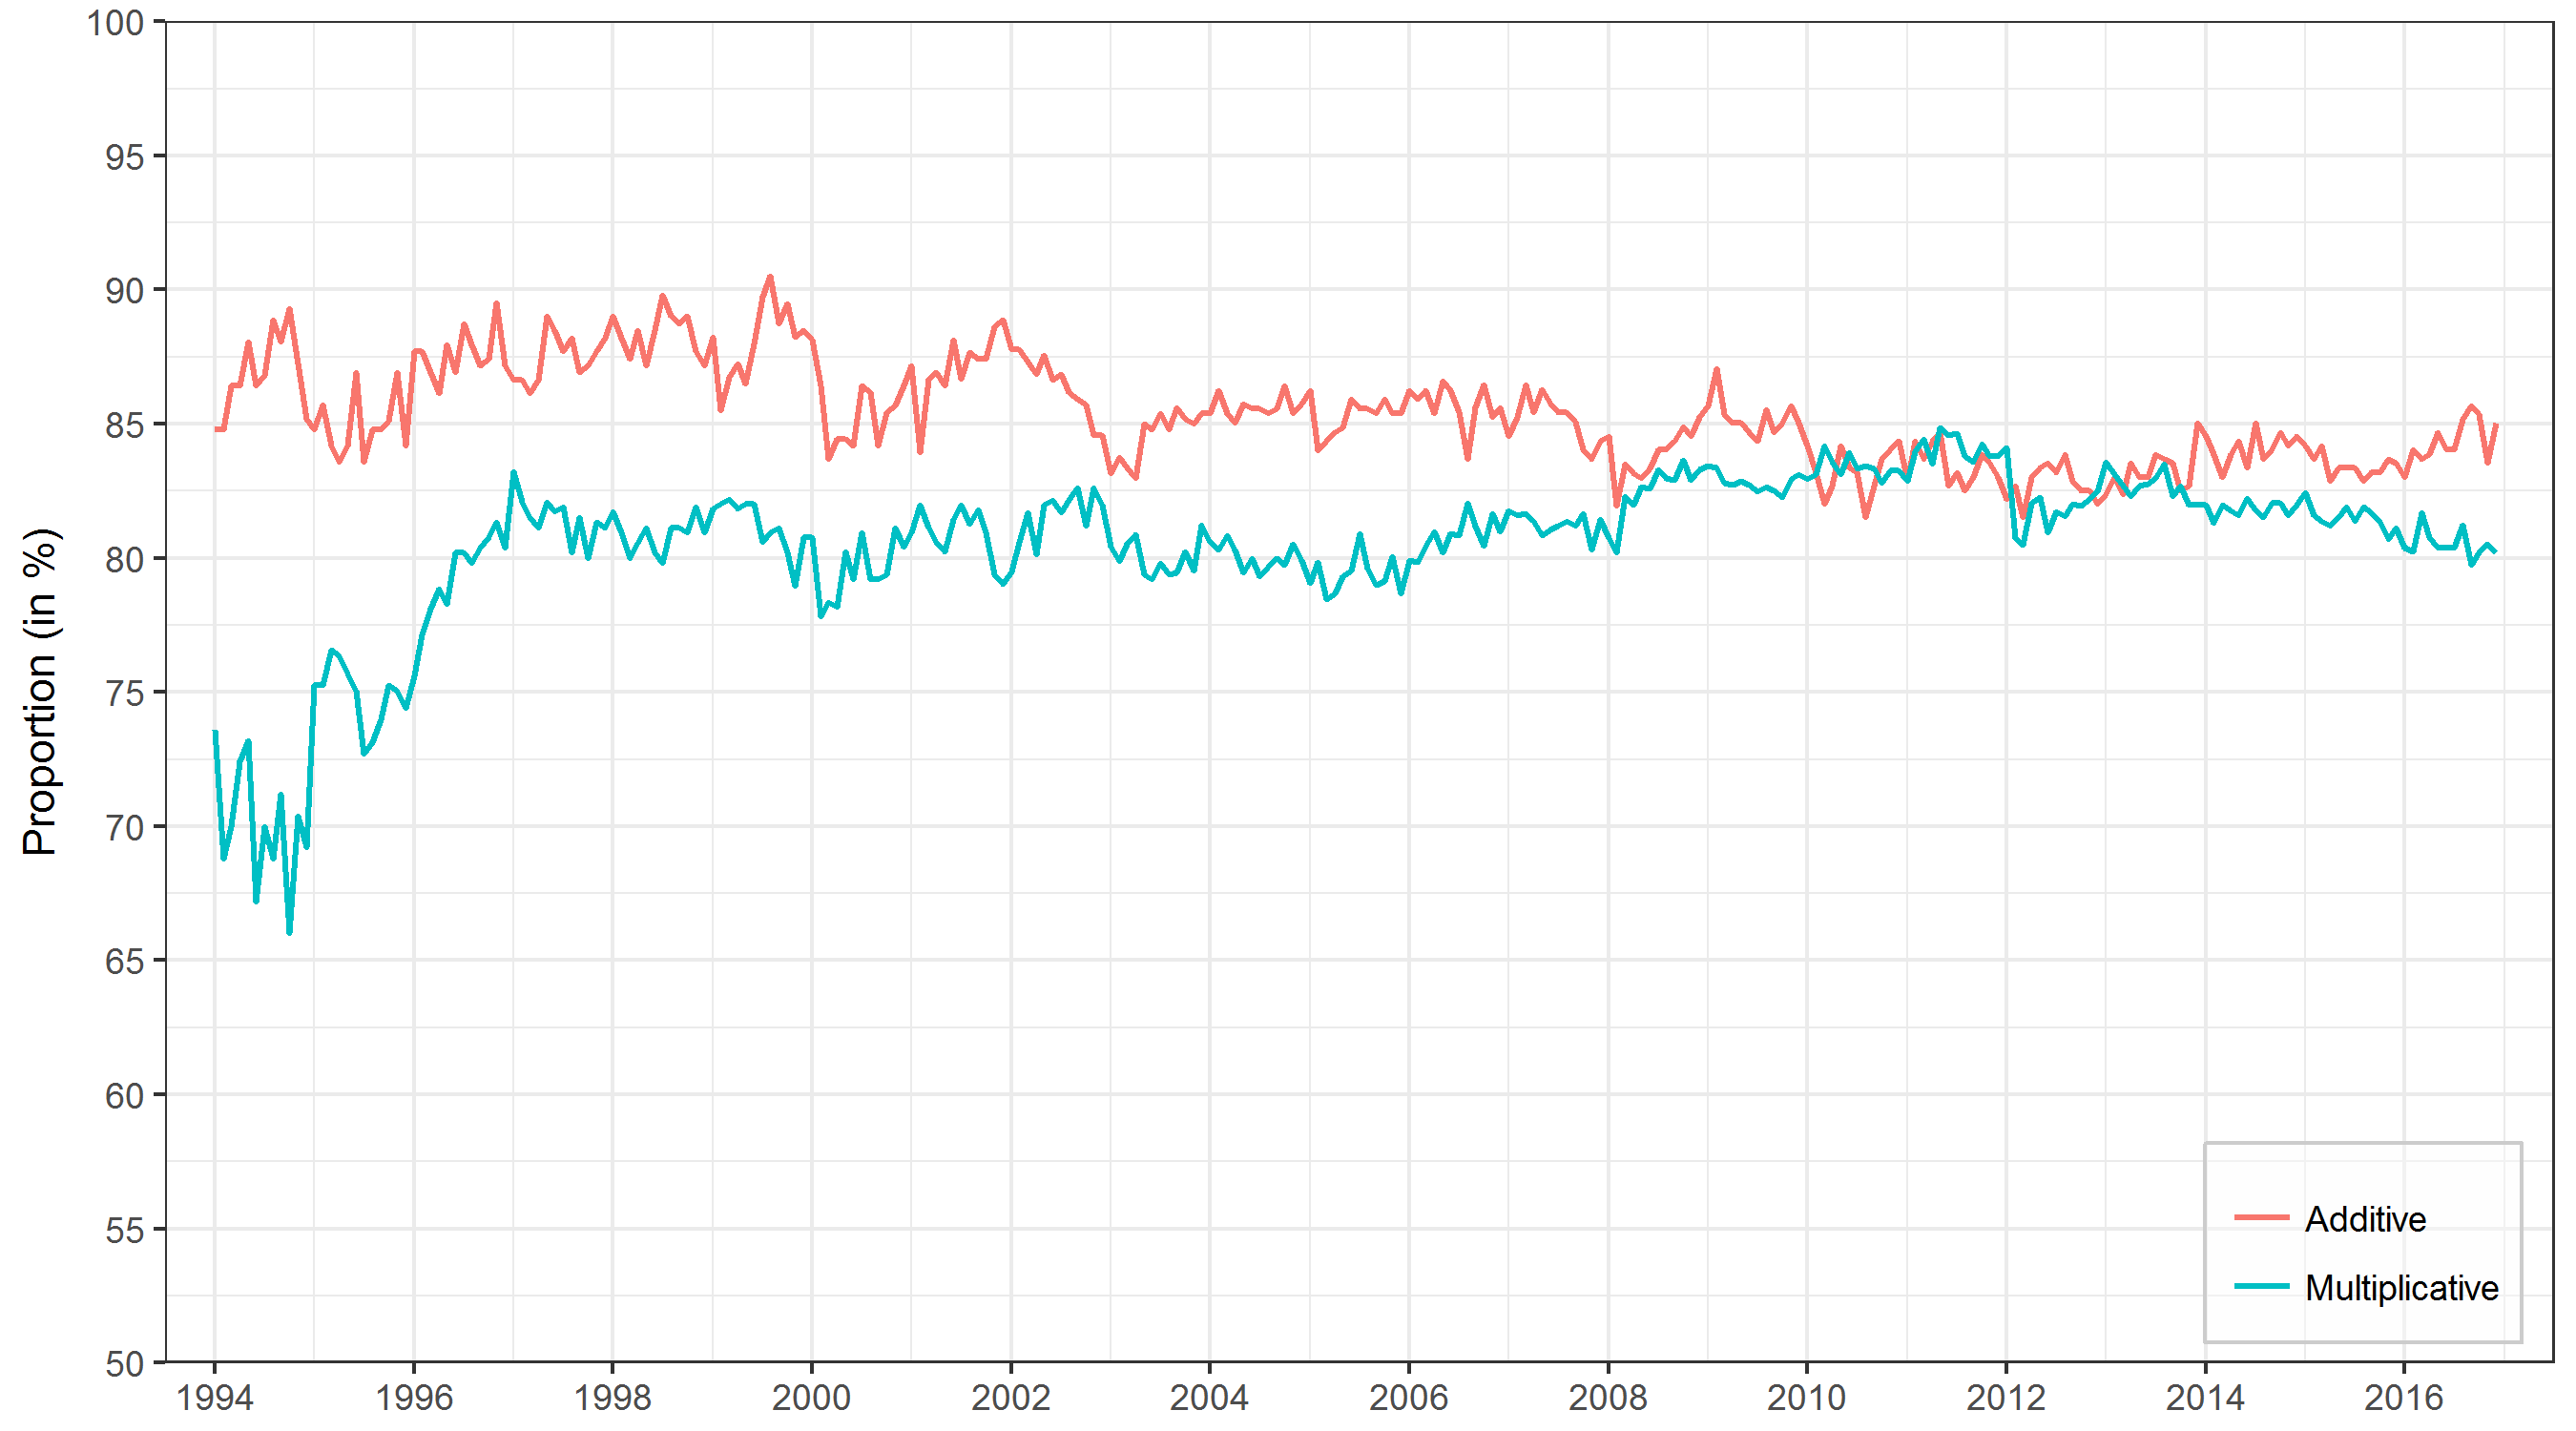
\includegraphics[width = \textwidth]{img/LYaicc.png}
\end{figure}
\end{frame}

\section{Outliers}
\begin{frame}{Outline}
\tableofcontents[currentsection, hideothersubsections]
\end{frame}

\begin{frame}{Usuals outliers}
\centering
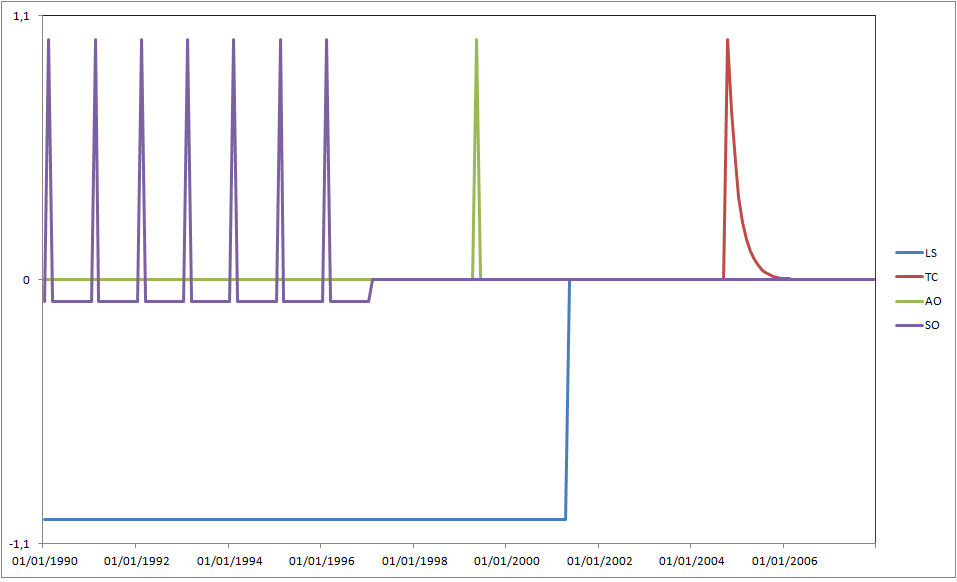
\includegraphics[width = \textwidth]{img/Outliers.png}
\end{frame}

\subsection{Methodology of the study}
\begin{frame}{Methodology}

\begin{enumerate}
	\item Simulations done on the European IPIs, NACE2, 4 digits;
	\item We keep the 12 first years of observations. The decomposition model, the ARIMA model, outliers and TD effect are identified and estimated on the 12 years. The decomposition model and the ARIMA model are kept fixed for the study;
	\item<2-> The rupture will be introduced at observation 49 so:
	\begin{itemize}
	  \item<2-> The series is corrected for any outlier detected at observations 49 to 50 (one year).
	  \item<2-> To facilitate the estimations and the comparisons, each series is rebased at 100 at observation 49;
	\end{itemize}
	\item<3-> The rupture is introduced with a level 10 for an additive model and 1.1 for a multiplicative model;
	\item<3-> The estimation of the outlier coefficient is done adding each time a new observation. Thus, for a 12-year series, we obtain $12 \times 12 - 48 = 96$ estimations of the coefficient.
	\item<4-> We assume that the convergence is reached when $\left\lvert\frac{\text{estimated value}}{\text{last estimated value}}-1\right\rvert < 5\;\%$
\end{enumerate}
\end{frame}


\subsection{Example}
\begin{frame}{Example}
\footnotesize
IPI IT-1413 (manufacture of other outerwear): AO introduced in January 1995. 
\normalsize
\begin{figure}
\centering
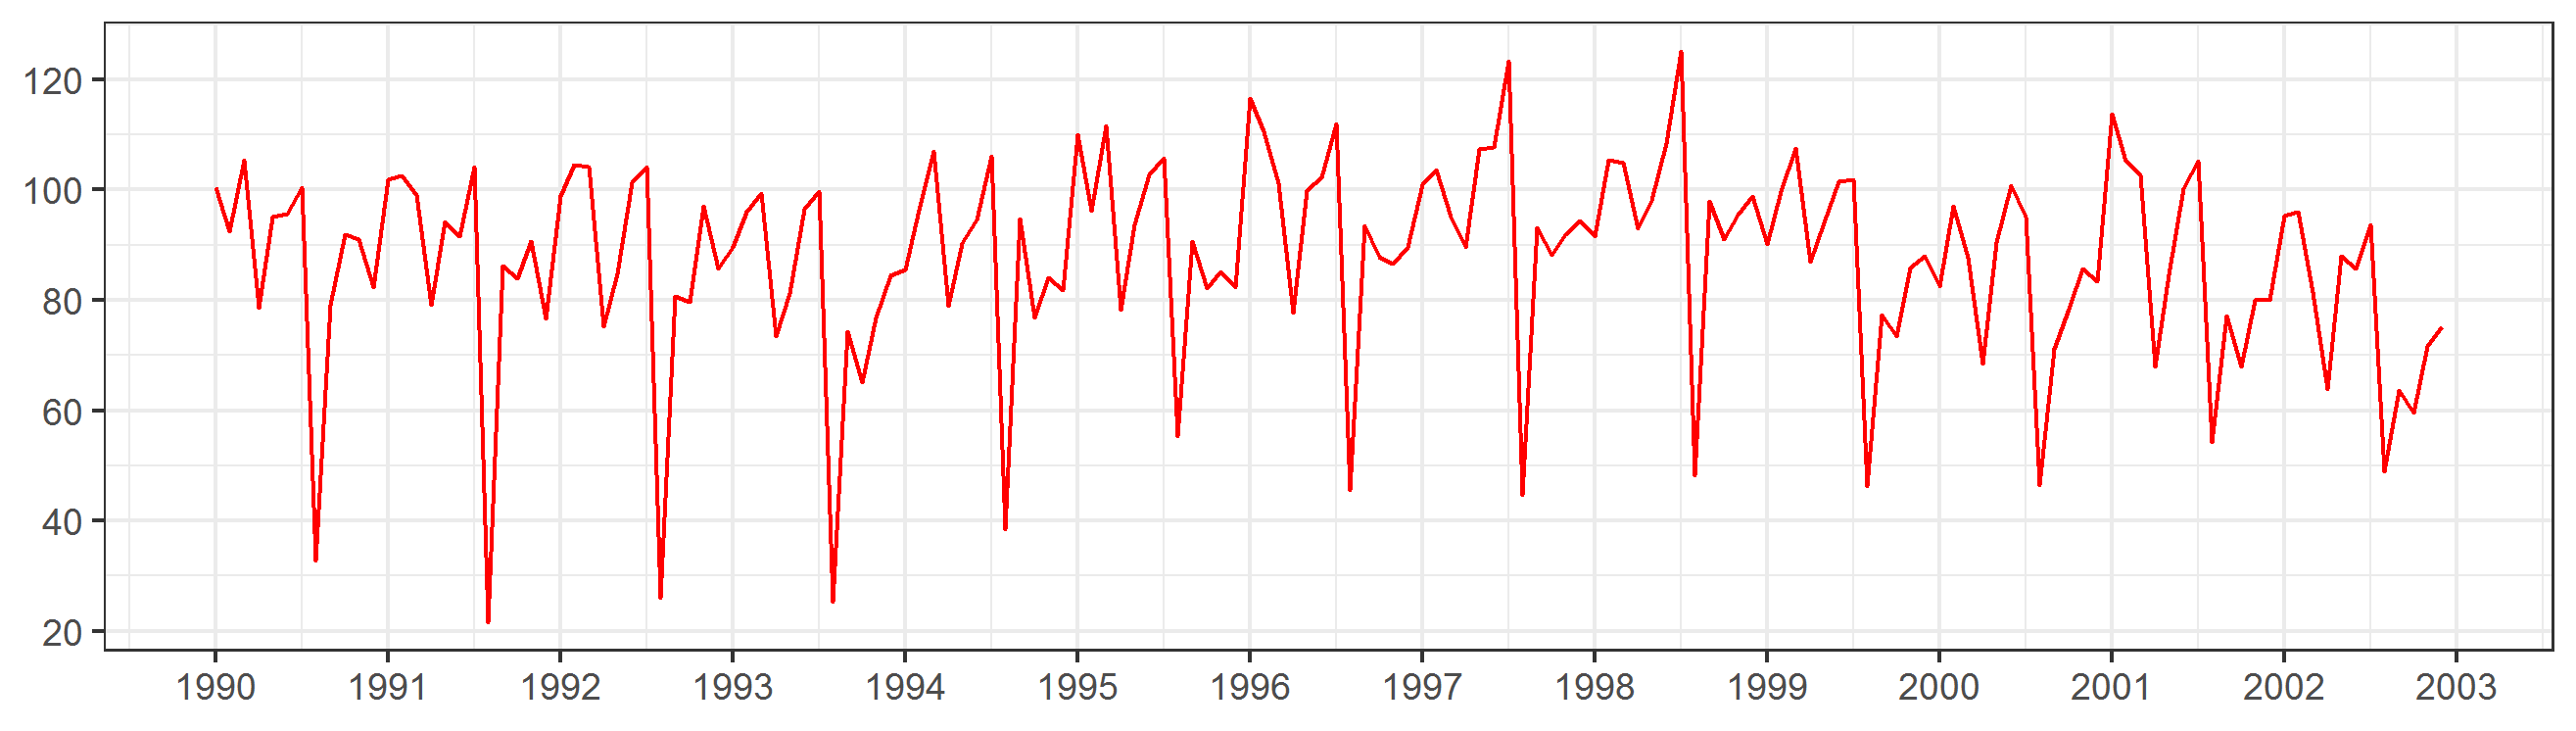
\includegraphics[width=0.9\textwidth]{img/AO_ipi_it1413_y.png}

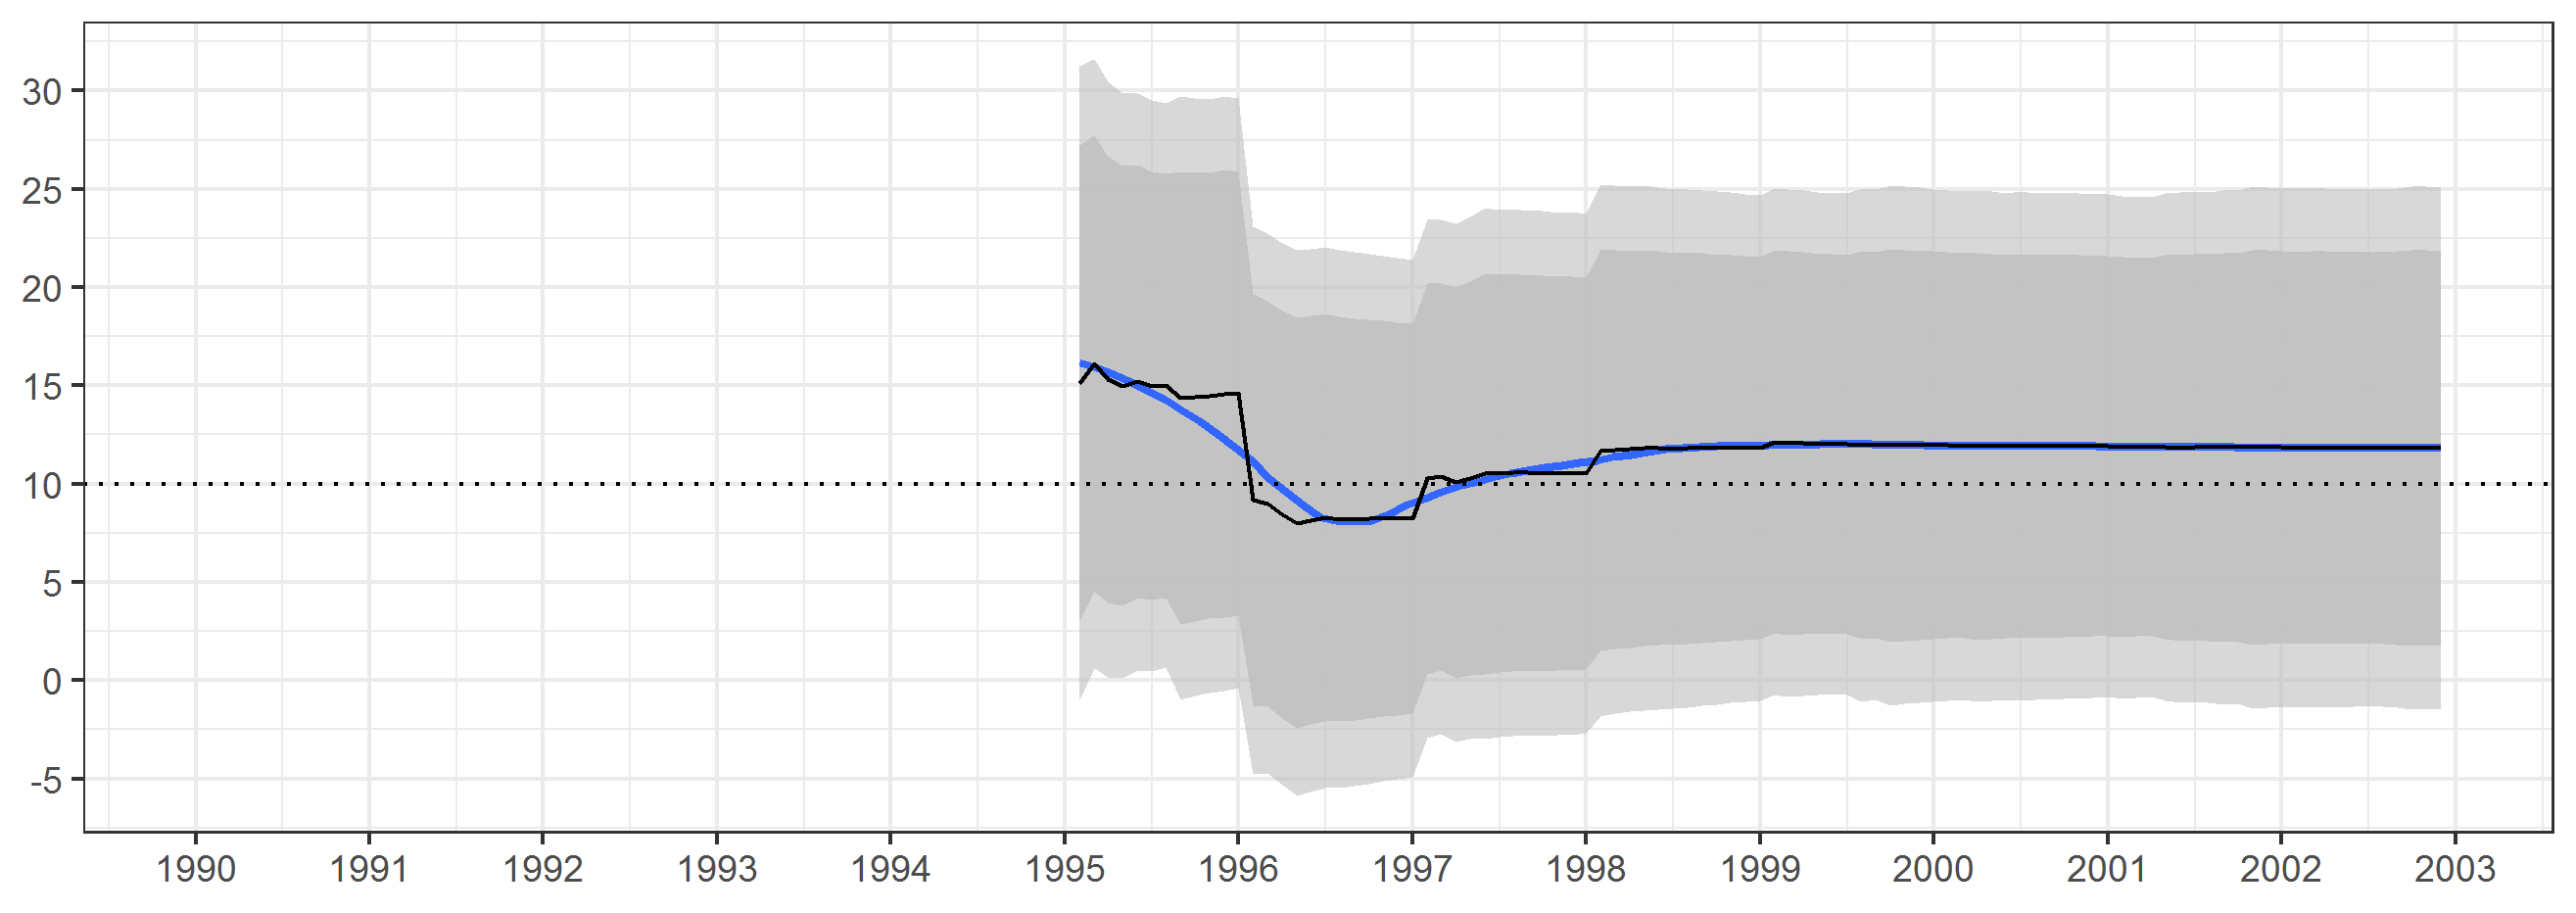
\includegraphics[width=0.9\textwidth]{img/AO_ipi_it1413_est.png}
\end{figure}
\end{frame}


\subsection{Results}
\begin{frame}{Results: A rather slow convergence\ldots{}}
\centering
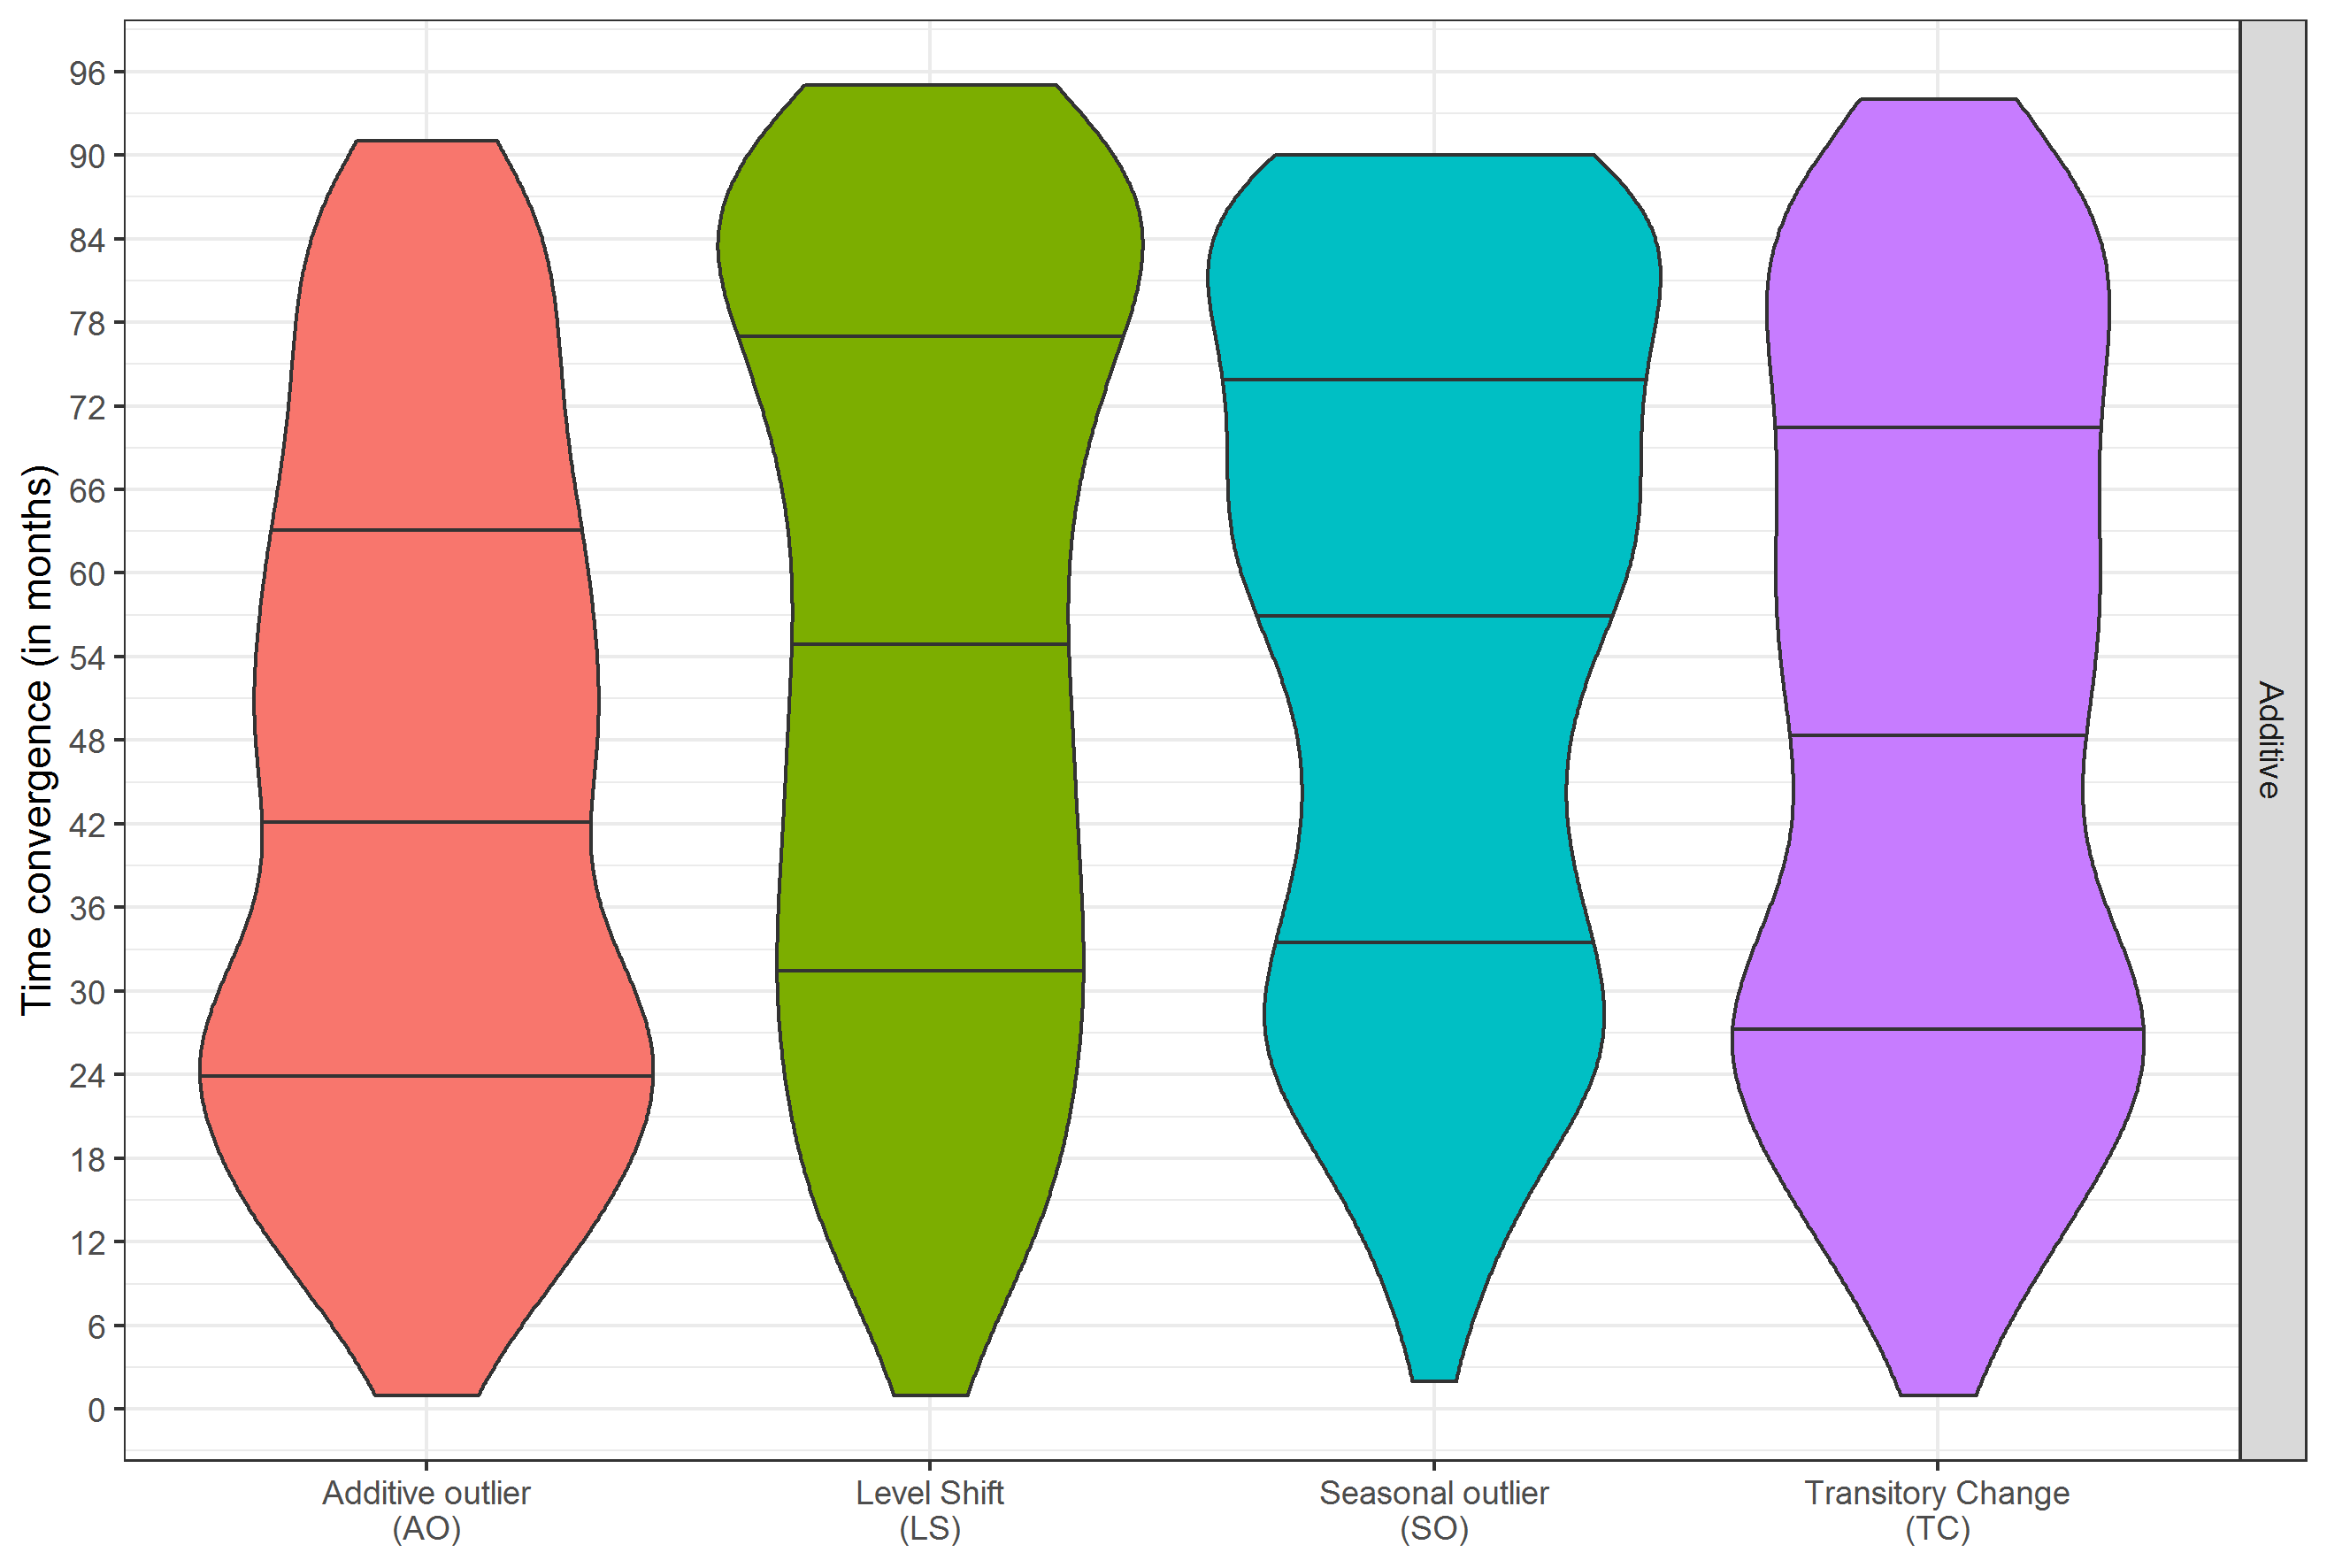
\includegraphics[width=0.9\textwidth]{img/outliers_convergence_additif_5.png}\\
\end{frame}

\begin{frame}{\ldots{} And not always to the correct value}

\begin{table}
\begin{center}
\footnotesize
\begin{tabular}{lccccc}
\hline
\rule{0pt}{3ex}  & Minimum & 25 \% & 50 \% & 75 \% & Maximum\\
\hline
& & & & & \\
\bf{Additive Models} & & & & & \\
& & & & & \\
Additive outlier (AO) & -11.6 & 7.8 & 11.1 & 14.2 & 36.9\\
Level Shift (LS) & -11.4 & 5.6 & 9.3 & 12.7 & 49.8\\
Seasonal outlier (SO) & -5.8 & 7.3 & 8.8 & 11.0 & 31.1\\
Transitory Change (TC) & -17.4 & 6.5 & 10.2 & 14.1 & 47.2\\
\hline
\end{tabular}
\normalsize
\end{center}
\end{table}
\end{frame}

\section{Identification of the ARIMA model}
\begin{frame}{Outline}
\tableofcontents[currentsection, hideothersubsections]
\end{frame}

\begin{frame}{Identification of two ``equivalent'' models}

We use the same leap year regressor in 2 different, but mathematically equivalent, forms:
\begin{enumerate}
\def\labelenumi{\arabic{enumi}.}
\item   The leap year regressor is added in the trading-day regressors;
\item   The leap year regressor is added as an external (not calendar) regressor.
\end{enumerate}

\(\rightarrow\) and we run an AMI.

\end{frame}

\begin{frame}{An example where we get quite different models}
\centering
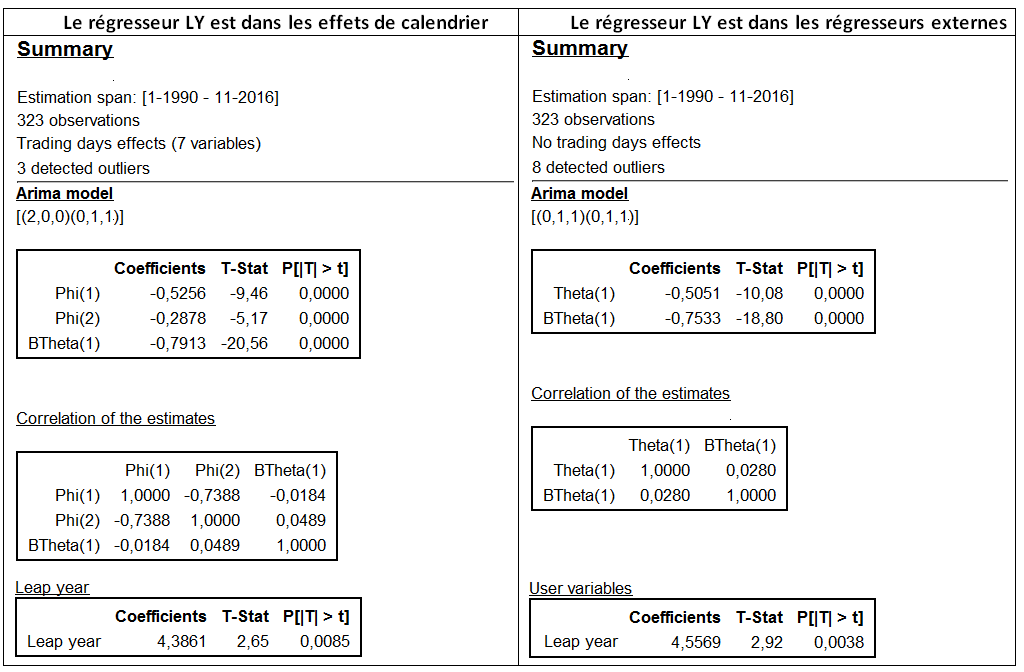
\includegraphics[width = \textwidth]{img/CholeskyRF241.png}
\end{frame}

\section{Conclusion}
\begin{frame}{Conclusions}

\bcinfo These simulations are certainly questionable and can be improved; but they highlight the instability of Reg-ARIMA models often used as black boxes.

\medskip  \pause
\bcsmbh These instabilities usually have a limited effect on the SCA series\dots \bcsmmh but might have an impact on the
short term history and on revisions.

\medskip  \pause
\bcattention Automatic algorithms in X-13ARIMA-SEATS and TRAMO-SEATS are important and  useful but do not prevent you from a precise specification of the model for each series.

\medskip  \pause
\bcattention Remains at the end that it is difficult to estimate some effects. For example, the estimation of a LY effect requires a long series; but in this case it will be difficult to suppose ONE Arima model for the time span.


\end{frame}


\end{document}